\begin{block}{Problem Statement}
  Samantha has a total credit limit of \$8,000. She chooses a target utilization ratio at or below \textbf{15\%} to keep her reported balances low.

  What is the maximum total balance Samantha can carry across her credit cards?
\end{block}

\vspace{0.8em}
\centering
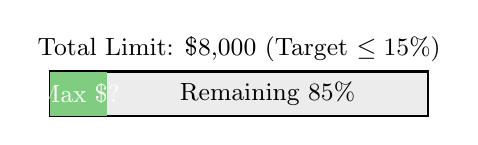
\begin{tikzpicture}[scale=0.8]
  \draw[thick, fill=gray!15] (0,0) rectangle (6,0.7);
  \fill[green!60!black!50] (0,0) rectangle (0.9,0.7);
  \node at (0.45,0.35) {\color{white}\small Max \$?};
  \node at (3.45,0.35) {\small Remaining 85\%};
  \node[above] at (3,0.7) {\small Total Limit: \$8,000 (Target $\le 15\%$)};
\end{tikzpicture}
